\begingroup
\setstretch{1}
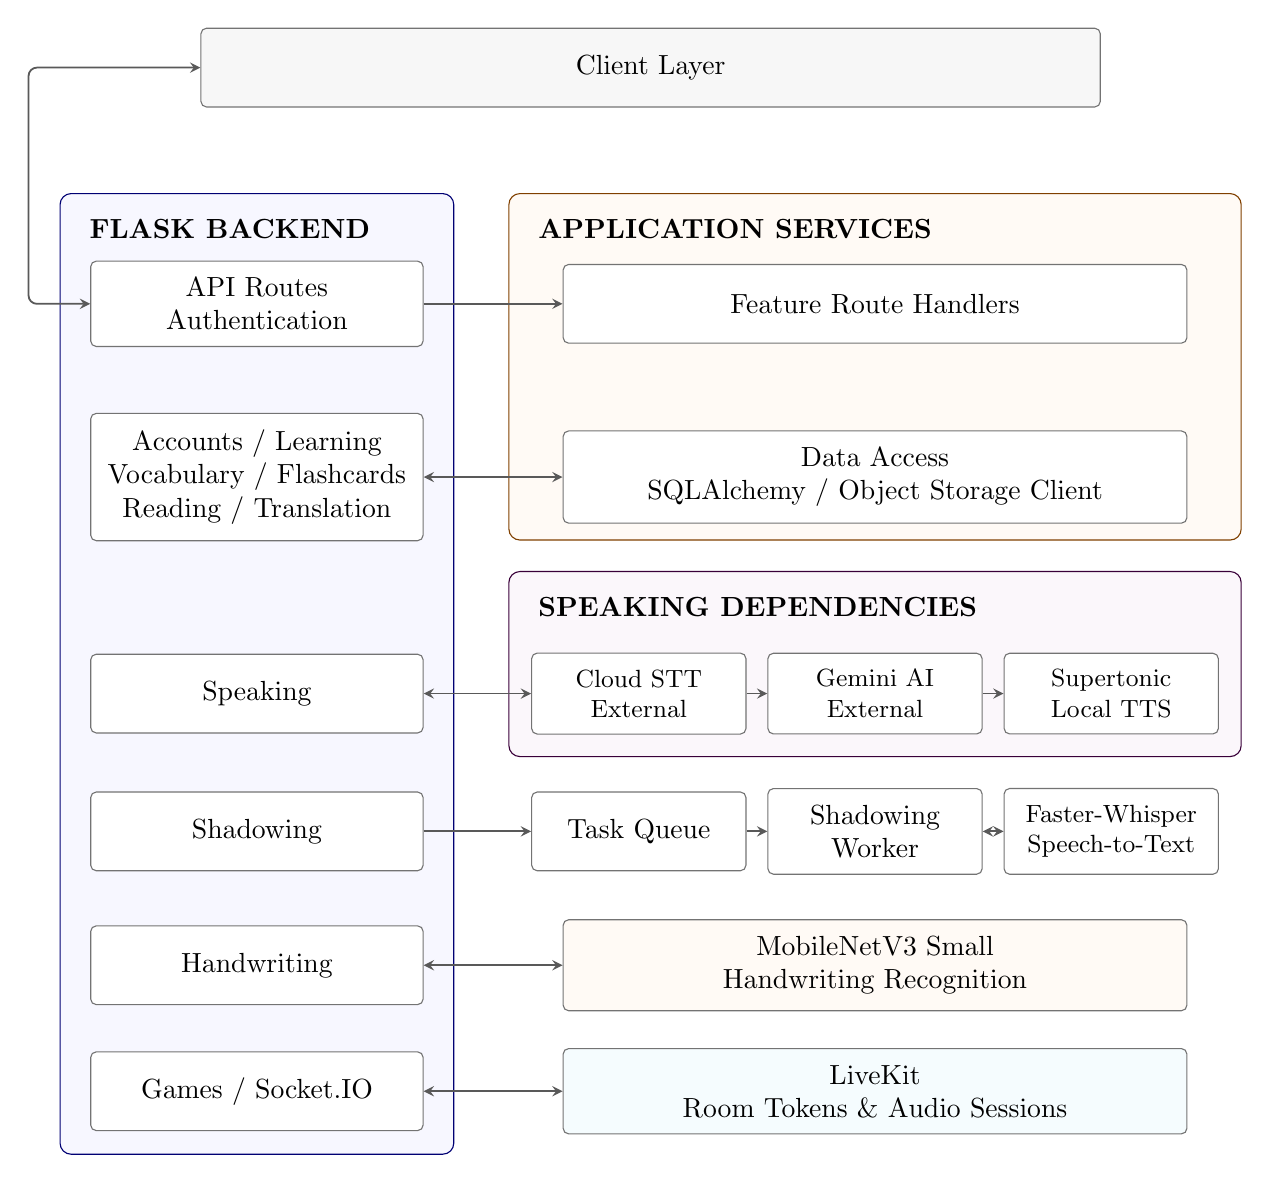
\begin{tikzpicture}[
box/.style={draw=black!55,rounded corners=2pt,fill=white,text width=3.8cm,minimum height=1cm,inner sep=6pt,align=center,font=\fontsize{10}{12}\selectfont},
title/.style={anchor=north west,font=\fontsize{10}{12}\selectfont\bfseries},
link/.style={<->,>=stealth,draw=black!65,line width=.65pt,rounded corners=3pt},
task/.style={->,>=stealth,draw=black!65,line width=.65pt,rounded corners=3pt}]

\node[box,text width=11cm,fill=black!3] (client) at (0,0) {Client Layer};
\draw[rounded corners,draw=blue!45!black,fill=blue!3] (-7.5,-1.6) rectangle (-2.5,-13.8);
\node[title] at (-7.25,-1.8) {FLASK BACKEND};
\node[box] (api) at (-5,-3) {API Routes\\Authentication};
\node[box] (core) at (-5,-5.2) {Accounts / Learning\\Vocabulary / Flashcards\\Reading / Translation};
\node[box] (speaking) at (-5,-7.95) {Speaking};
\node[box] (shadow) at (-5,-9.7) {Shadowing};
\node[box] (hand) at (-5,-11.4) {Handwriting};
\node[box] (games) at (-5,-13) {Games / Socket.IO};
\draw[link] (client.west) -- (-7.9,0) -- (-7.9,-3) -- (api.west);
\draw[rounded corners,draw=orange!50!black,fill=orange!4] (-1.8,-1.6) rectangle (7.5,-6);
\node[title] at (-1.55,-1.8) {APPLICATION SERVICES};
\node[box,text width=7.5cm] (handlers) at (2.85,-3) {Feature Route Handlers};
\node[box,text width=7.5cm] (data) at (2.85,-5.2) {Data Access\\SQLAlchemy / Object Storage Client};
\draw[task] (api.east) -- (handlers.west);
\draw[link] (core.east) -- (data.west);
\draw[rounded corners,draw=violet!45!black,fill=violet!3] (-1.8,-6.4) rectangle (7.5,-8.75);
\node[title] at (-1.55,-6.6) {SPEAKING DEPENDENCIES};
\node[box,text width=2.3cm,font=\fontsize{9}{11}\selectfont] (stt) at (-.15,-7.95) {Cloud STT\\External};
\node[box,text width=2.3cm,font=\fontsize{9}{11}\selectfont] (ai) at (2.85,-7.95) {Gemini AI\\External};
\node[box,text width=2.3cm,font=\fontsize{9}{11}\selectfont] (tts) at (5.85,-7.95) {Supertonic\\Local TTS};
\draw[link] (speaking.east) -- (stt.west);
\draw[task] (stt.east) -- (ai.west);
\draw[task] (ai.east) -- (tts.west);
\node[box,text width=2.3cm] (q) at (-.15,-9.7) {Task Queue};
\node[box,text width=2.3cm] (w) at (2.85,-9.7) {Shadowing Worker};
\node[box,text width=2.3cm,font=\fontsize{9}{11}\selectfont] (whisper) at (5.85,-9.7) {Faster-Whisper\\Speech-to-Text};
\draw[task] (shadow.east) -- (q.west);
\draw[task] (q.east) -- (w.west);
\draw[link] (w.east) -- (whisper.west);
\node[box,text width=7.5cm,fill=orange!4] (model) at (2.85,-11.4) {MobileNetV3 Small\\Handwriting Recognition};
\draw[link] (hand.east) -- (model.west);
\node[box,text width=7.5cm,fill=cyan!4] (live) at (2.85,-13) {LiveKit\\Room Tokens \& Audio Sessions};
\draw[link] (games.east) -- (live.west);
\end{tikzpicture}
\endgroup
